% !TeX root = ../main.tex
\section{Runtime data representation}

We've talked a lot about what values \emph{mean}. Now let's talk about what they
literally \emph{are}, once a program is actually running: bits, in memory, at some
address, with some layout. This is the layer where a type system's promises meet
physical hardware, and where a lot of language-design decisions (dynamic vs.\ static
typing, whether integers can be arbitrarily large, how expensive a function call is)
get paid for or profited from.

\subsection{tagged values: boxing vs.\ unboxing}

A statically-typed compiled language usually knows, at compile time, exactly what type
every value has, so it doesn't need to store that information at runtime; a machine
word holding an \texttt{int} is just the bits of the integer, full stop. A
dynamically-typed language doesn't have that luxury: a variable can hold an integer
today and a string tomorrow, so \emph{something} at runtime has to be able to answer
``what kind of value is this bit pattern?''. The answer is a \textbf{tag}: a small
piece of metadata, stored alongside (or packed into) the value, that identifies its
type.

\begin{definition}[Boxed representation]
A value is \textbf{boxed} when it's represented as a pointer to a heap-allocated
object that itself contains the tag and the actual data. Reading a boxed value costs
a pointer dereference (and the object had to be allocated somewhere, at some point).
\end{definition}

\begin{definition}[Unboxed / immediate representation]
A value is \textbf{unboxed} (or \textbf{immediate}) when the value itself, tag
included, fits directly in a machine word, no heap allocation and no extra
indirection required to read it.
\end{definition}

The classic trick for making small integers unboxed even in a language where
everything else is boxed (Python's arbitrary-precision ints, Ruby, many Lisp/Scheme
implementations) is the \textbf{tagged pointer}. A pointer to a heap object is always
word-aligned, so its low bits (2 or 3 of them, depending on word size and alignment)
are always zero for a real pointer. That means those bits are free real estate: steal
the lowest bit to mean ``this is not a pointer, it's a small integer, and the rest of
the word is the integer's value, shifted left by one.''

\begin{center}
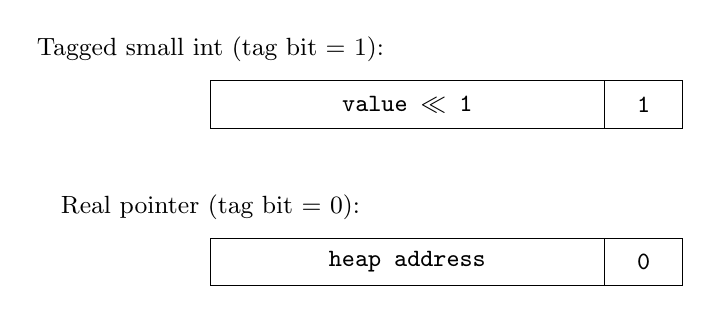
\begin{tikzpicture}[node distance=0cm]
  \node (label1) [font=\small] at (0,1) {Tagged small int (tag bit = 1):};
  \draw (0,0) rectangle (6,0.6);
  \draw (5,0) -- (5,0.6);
  \node at (2.5,0.3) [font=\ttfamily\small] {value $\ll$ 1};
  \node at (5.5,0.3) [font=\ttfamily\small] {1};

  \node (label2) [font=\small] at (0,-1) {Real pointer (tag bit = 0):};
  \draw (0,-2) rectangle (6,-1.4);
  \draw (5,-2) -- (5,-1.4);
  \node at (2.5,-1.7) [font=\ttfamily\small] {heap address};
  \node at (5.5,-1.7) [font=\ttfamily\small] {0};
\end{tikzpicture}
\end{center}

Checking whether a word holds a small int or a pointer is one bitwise \texttt{AND} and
a comparison; no allocation, no dereference. This is why arithmetic on small integers
in dynamically-typed runtimes doesn't cost a heap allocation per operation, it's the
main reason the trick exists. The cost shows up only when a value needs to escape that
immediate range (a Python integer bigger than a machine word, an arbitrary object): then
you fall back to a real, boxed, heap-allocated representation, with the pointer
indirection and allocation cost that boxing implies.

\begin{remark}
Boxing everything is simpler to implement uniformly (every value is ``a pointer to a
tagged object'', full stop, no special cases), but every arithmetic operation now costs
an allocation and a dereference. Unboxing small, common cases (integers, booleans,
sometimes floats) is more implementation work, but it's the difference between
\texttt{i++} being a machine instruction and \texttt{i++} being a heap allocation.
\end{remark}

\subsection{composite values}

\subsubsection{records and objects}

For a statically-typed language, a record's field layout is known entirely at compile
time: the compiler assigns each field a fixed byte offset from the start of the
record, and reading \texttt{p.y} compiles down to ``load 8 bytes starting at
\texttt{address\_of(p) + offset\_of(y)}'', no runtime lookup involved.

\begin{lstlisting}[language=C]
struct Point { double x; double y; };  /* offset(x) = 0, offset(y) = 8 */
\end{lstlisting}

A dynamically-typed language with objects whose shape can change at runtime (adding or
removing fields on the fly, as in JavaScript or Python) can't fix offsets once and for
all at compile time, because two objects that look like they have ``the same type''
from the program's point of view might not, structurally, at any given moment. The
common trick (V8's \emph{hidden classes}, Python's per-object \texttt{\_\_dict\_\_}) is
either: (a) a dictionary mapping field names to values, looked up by hashing the name
at every access, or (b) an inferred ``shape''/hidden class that's computed and cached
the first time a particular field layout is seen, so that objects with the same
observed shape can share fast, offset-based access after the first lookup. Either way,
you're paying \emph{something} (a hash lookup, or a shape check) that a statically-typed
language with fixed offsets doesn't have to pay.

\subsubsection{arrays}

An array is the simplest case: elements of the same size, laid out contiguously, so
that indexing is arithmetic, not search.
\[
  \mathrm{address}(a[i]) = \mathrm{base}(a) + i \times \mathrm{size}(\mathrm{element})
\]
That's an O(1) formula, one multiply and one add, which is the entire reason arrays are
the default ``fast, random-access sequence'' data structure. The place a \emph{bounds
check} fits in is right before that formula is used: a safe language inserts
\texttt{if (i < 0 || i >= length) raise IndexError} before computing the address, an
unsafe one (raw C arrays) doesn't, and just computes the address anyway, undefined
behaviour and all, if $i$ is out of range.

\subsubsection{sum / variant types}

An algebraic sum type (recall the recursive/algebraic types discussion:
$\mathbf{List}\ \tau = \mu\alpha.\ \unit + (\tau \times \alpha)$, or an
\texttt{enum}/\texttt{union} in a language with tagged unions) needs, at runtime,
exactly the same idea as our dynamic-typing tag from before, but scoped to one type
instead of ``everything'': a small \textbf{tag word} identifying which variant this
value is, followed by however much storage the largest variant's payload needs (sized
to fit whichever variant is actually present).

\begin{center}
\begin{tikzpicture}[node distance=0cm]
\node[draw,minimum width=1.4cm,minimum height=0.7cm] (tag) at (0,0) {tag};
\node[draw,minimum width=3.5cm,minimum height=0.7cm,right=0cm of tag] (payload)
  {payload (variant-sized)};
\node[below=0.15cm of tag, font=\scriptsize] {e.g.\ \texttt{0 = Nil}, \texttt{1 = Cons}};
\node[below=0.15cm of payload, font=\scriptsize] {e.g.\ \texttt{Cons}: head value + tail pointer};
\end{tikzpicture}
\end{center}
\texttt{Nil}'s tag word says ``there's no payload to look at''; \texttt{Cons}'s tag
word says ``the payload is a head value and a pointer to the tail''. Pattern matching
compiles down to: read the tag, jump to the code for that variant, and only then
interpret the payload bytes according to that variant's known layout.

\subsection{closures: code plus captured environment}

Recall from the environments and scoping discussion that a closure is a function
paired with the environment it was defined in, so that it can still see its free
variables after that defining scope has, in principle, ended. At runtime this has to be
an actual, concrete data structure: a \textbf{closure record} holding (1) a pointer to
the function's compiled code, and (2) a pointer to (or an inline array of) the captured
environment, the bindings for the free variables the function body refers to.

\begin{center}
\begin{tikzpicture}[node distance=0cm]
\node[draw,minimum width=2.6cm,minimum height=0.7cm] (code) at (0,0) {code pointer};
\node[draw,minimum width=2.6cm,minimum height=0.7cm,right=0cm of code] (env)
  {env pointer};
\node[below=1.1cm of env, draw, minimum width=3cm, align=left, font=\ttfamily\small]
  (envbox) {n = 5\\ threshold = 10};
\draw[->] (env.south) -- (envbox.north);
\end{tikzpicture}
\end{center}

\begin{example}[A counter closure]
\begin{lstlisting}[language=Python]
def make_counter(start):
    n = start
    def bump():
        nonlocal n
        n += 1
        return n
    return bump
\end{lstlisting}
Calling \texttt{make\_counter(5)} allocates one environment record holding
\texttt{n = 5}, and returns a closure record pointing to \texttt{bump}'s compiled code
plus that environment. Every call to the returned closure runs the same code pointer
but against that same captured environment, that's exactly what lets \texttt{n} persist
and increment across calls instead of resetting to 5 every time.
\end{example}

\subsection{activation records / stack frames}

Every (non-tail) function call needs somewhere to keep its local state while it runs,
and that somewhere is an \textbf{activation record} (a.k.a. stack frame), pushed onto
the call stack on entry and popped on return. A typical layout:

\begin{center}
\begin{tikzpicture}[node distance=0cm]
\node[draw,minimum width=3.6cm] (ra) at (0,0) {return address};
\node[draw,minimum width=3.6cm,below=0cm of ra] (fp) {saved frame pointer};
\node[draw,minimum width=3.6cm,below=0cm of fp] (params) {parameters};
\node[draw,minimum width=3.6cm,below=0cm of params] (locals) {locals};
\node[left=0.3cm of ra, font=\small] {higher addresses};
\node[left=0.3cm of locals, font=\small] {lower addresses};
\end{tikzpicture}
\end{center}

\begin{itemize}
  \item \textbf{Return address}: where execution resumes in the caller once this call
    returns.
  \item \textbf{Saved frame pointer}: the caller's frame pointer, so it can be restored
    on return (this is what lets you walk the stack, frame by frame, for a debugger or
    a stack trace).
  \item \textbf{Parameters}: the arguments this call was invoked with.
  \item \textbf{Locals}: this call's own local variables, live only for the duration of
    this activation.
\end{itemize}

\begin{example}[Three frames during \texttt{fact(3)}]
\begin{lstlisting}[language=C]
int fact(int n) {
    if (n == 0) return 1;
    return n * fact(n - 1);
}
\end{lstlisting}
Mid-way through evaluating \texttt{fact(3)}, the call stack (growing downward) looks
like:
\begin{center}
\begin{tikzpicture}[node distance=0cm]
\node[draw,minimum width=4.2cm,fill=gray!10] (f0) at (0,0)
  {\texttt{fact(3)}: n=3, waiting on fact(2)};
\node[draw,minimum width=4.2cm,fill=gray!10,below=0cm of f0] (f1)
  {\texttt{fact(2)}: n=2, waiting on fact(1)};
\node[draw,minimum width=4.2cm,fill=gray!10,below=0cm of f1] (f2)
  {\texttt{fact(1)}: n=1, waiting on fact(0)};
\node[draw,minimum width=4.2cm,below=0cm of f2] (f3)
  {\texttt{fact(0)}: n=0, about to return 1};
\node[left=0.3cm of f0, font=\small] {bottom of stack (oldest)};
\node[left=0.3cm of f3, font=\small] {top of stack (newest)};
\end{tikzpicture}
\end{center}
Each frame is independently holding its own \texttt{n}; that's precisely why recursion
works without the calls stomping on each other's variables. \texttt{fact(0)} returns 1,
its frame pops, \texttt{fact(1)} resumes with that 1, computes \texttt{1*1=1}, returns,
pops, and so on back up to \texttt{fact(3)} finally computing \texttt{3*2*1=6}.
\end{example}

\subsection{reaching non-local scopes: static links vs.\ displays}

If a function is nested inside another (as in Pascal, or any language with true nested
function definitions) and refers to a variable from an \emph{enclosing}, non-local
scope, the runtime needs a way to find that enclosing frame from the inner one. Two
classic techniques:

\begin{itemize}
  \item \textbf{Static link}: every frame carries one extra pointer, to the frame of
    the lexically enclosing function's most recent activation. Looking up a variable
    $k$ scopes out means following $k$ static links. Simple to set up, but a lookup
    $k$ levels up costs $O(k)$ pointer chases.
  \item \textbf{Display}: instead of one static link per frame, maintain a single
    global array indexed by lexical nesting depth, where slot $d$ always holds a
    pointer to the current, innermost active frame at nesting depth $d$. Looking up a
    variable at depth $d$ is one array access, $O(1)$, at the cost of updating the
    display array on every call and return.
\end{itemize}
Static links are the more common choice in practice (simpler bookkeeping, and deep
nesting is rare enough that $O(k)$ chases rarely matter); displays trade a bit of
call/return overhead for guaranteed constant-time non-local access, which matters more
in languages or compilers that expect deep nesting to be common.

\subsection{Exercises}
\begin{itemize}
  \item Given a 64-bit word with 1 tag bit (0 = pointer, 1 = small int), what is the
    largest small integer representable in the immediate encoding, and what has to
    happen when an arithmetic operation's result would overflow that range?
  \item Trace by hand: for the \texttt{struct Point \{ double x; double y; \}} above,
    with \texttt{sizeof(double) == 8}, what byte offset does \texttt{p.y} compile to?
    What if a third field \texttt{double z;} were added before \texttt{y}?
  \item Draw the closure record and captured environment (as in the \texttt{make\_counter}
    example) after \texttt{c1 = make\_counter(5)} and \texttt{c2 = make\_counter(100)}
    have both been called once. Are \texttt{c1} and \texttt{c2}'s environments shared or
    separate? Why does that matter?
  \item Trace the call stack, frame by frame (as in the \texttt{fact(3)} example), for
    \texttt{fib(4)} where \texttt{fib(n) = fib(n-1) + fib(n-2)} for $n>1$, \texttt{fib(0)=0},
    \texttt{fib(1)=1}. How many frames exist at the deepest point?
  \item Think about it: why do bounds checks on array access, cheap as they individually
    are, sometimes get compiled away entirely by an optimizing compiler? What would the
    compiler need to prove about the index to justify removing the check?
  \item Compare static links and displays for a program with 5 levels of nested
    functions where the innermost function accesses a variable from the outermost
    scope on every iteration of a hot loop. Which technique would you pick, and why?
\end{itemize}
